\documentclass{article}
\usepackage[utf8]{inputenc}
\usepackage{float}

\title{Craters on the Moon}
\author{Oisín Peppard}
\date{April 2018}

\usepackage[a4paper, total={6in, 8in}]{geometry}
\usepackage{graphicx}


\begin{document}

\maketitle

\begin{abstract}
In this experiment, Lunar craters were examined using printed photographs. The heights of these craters were calculated using their measured diameters and the lengths of the shadows inside them. A linear relationship was observed between diameter and crater height. By relating crater heights to the energy of the impact causing them, we could estimate the masses of the asteroids that bombarded the Moon in its formation period. The range of values for these asteroid masses was $10^6$kg to $10^{13}$kg
By assuming a uniform distribution of craters, we estimate the number of craters greater than $16$km in diameter to be 3000
\end{abstract}


\section*{Theory and Method}
It is believed that the Earth's Moon was formed as a result of "the Theia Impact". An incident in the hadeon era of the early solar system approximately 4.5 billion years ago where an astronomical body the size of mars collided with the Earth. Since then, the Moon has been bombarded with asteroids leaving vast craters on its otherwise barren surface. Using high resolution images taken of the lunar surface, we calculate the diameter and height of these craters taking a sample of 21. The images are taken at any time other than a full moon, as this is the only way the craters will have shadows. Simple trigonometry is employed to calculate their heights by measuring the internal shadow with the zenith of the sun known. A description of this method is outlined in Fig 1.

\begin{figure}[h]
    \centering
    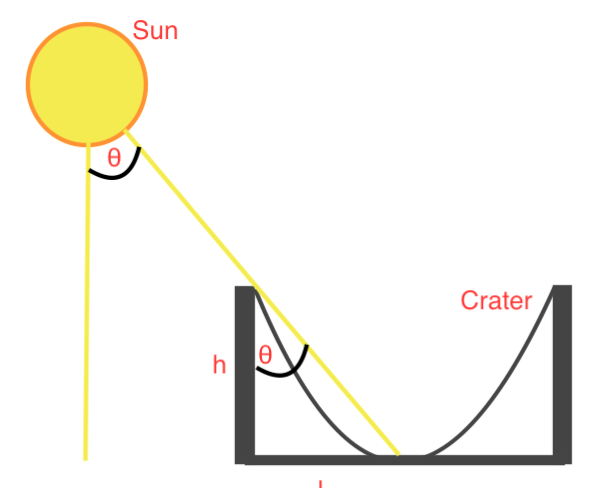
\includegraphics[width = 0.4\textwidth]{Diagram.png}
    \caption{Relationship of crater height $h$, shadow length $l$ and zenith angle $\theta$}
    \label{fig:Diagram}
\end{figure}

From this diagram we can see that the crater height $h$ can be given by: 
\begin{equation}
\frac{l}{\tan{\theta}}
\end{equation}
The diameters and shadow lengths of the craters were measured on the diagram with a ruler and their true dimensions $D$ and $l$ calculated using the length conversion factor provided with the image. For the larger crater, several diameter measurements were taken and an average used for the diameter. This is to compensate for the fact that the craters are not perfect circles. $h$ can then be calculated with (1) with the zenith angle of the sun $\theta$ given for each image. Crater height was plotted against diameter on a log-log plot. We use the following equation to relate diameter to the kinetic of the incident asteroid

\begin{equation}
    D = 2.5(\frac{E}{\rho g_M})^{\frac{1}{4}}
\end{equation}

where diameter is denoted $D$ in m, $E$ is the kinetic energy of the incident asteroid in Joules, $\rho$ the density of lunar rock $\approx 2 \times 10^3$ kg m\textsuperscript{-3}, and $g_M$ the acceleration due to gravity on the surface of the moon $\approx 1.62$ m s\textsuperscript{-2}. The dimension of the right side (with units) is 
\[(\frac{\frac{kg \times m \times m}{s^2}}{\frac{kg\times m}{m^3\times s^2}})^{\frac{1}{4}}\] 
which simplifies simply to m. Giving us the required dimension for the diameter.
The impact velocities of these impacts is taken to be 10~100 km/s. In the final part of this experiment we estimate the number of large impacts the moon has encountered by counting the number of craters with $D > 16$km. We also count the craters of size 8km, 4km and 2km, the relationship of these numbers is graphed linearly and logarithmically.

\section*{Results}

\begin{figure}[h!]
\centering
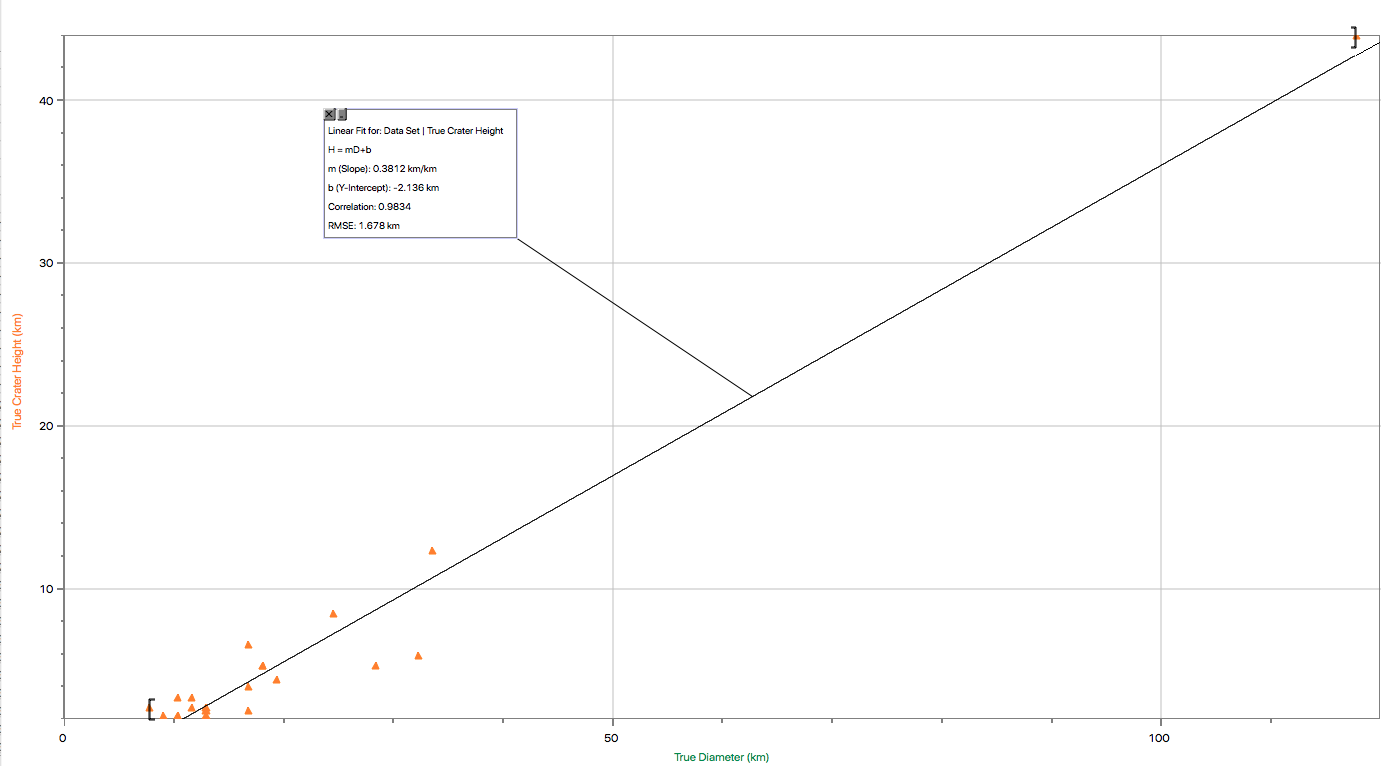
\includegraphics[width=0.85\textwidth]{1.png}
\caption{Crater Diameter vs. Crater height}
\end{figure}

\begin{figure}[H]
\centering
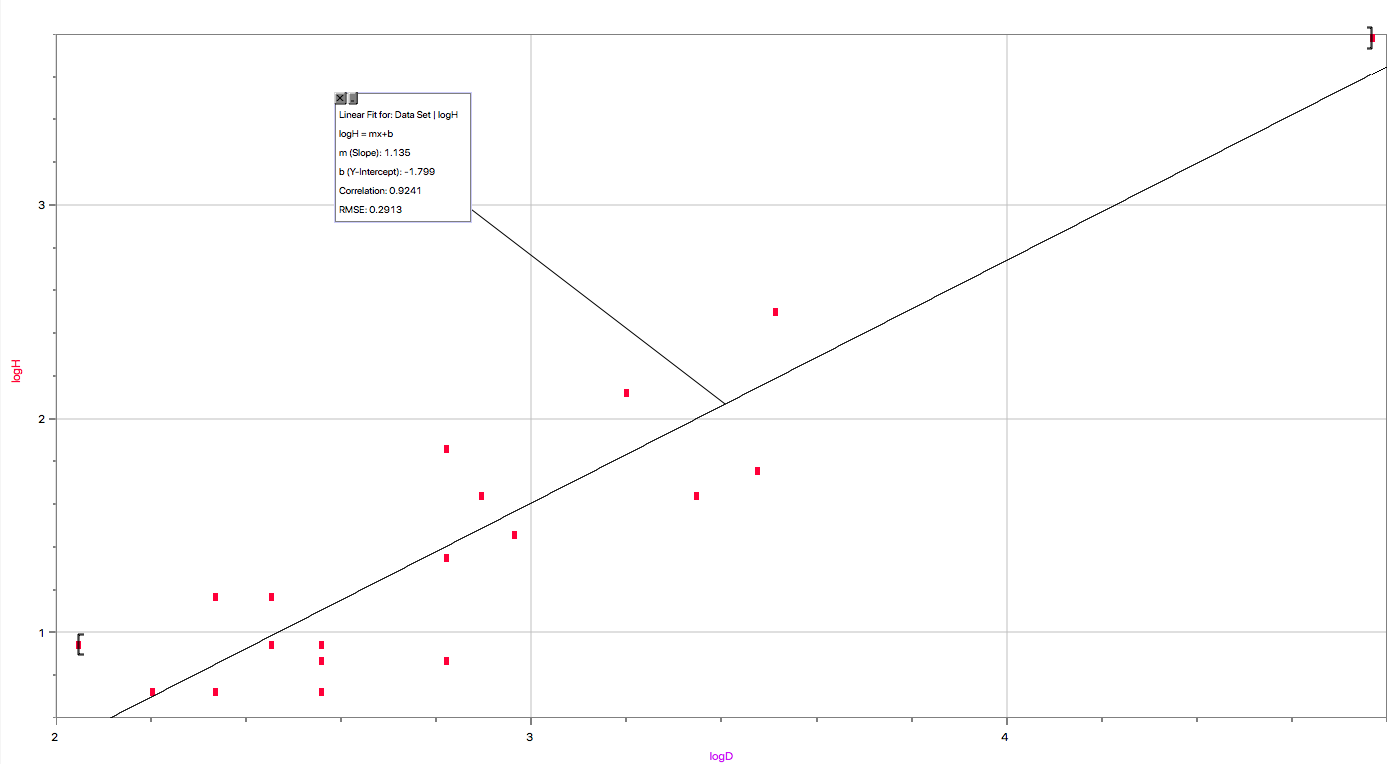
\includegraphics[width=0.85\textwidth]{2.png}
\caption{log-log plot for D vs. h}
\end{figure}

\begin{figure}[H]
    \centering
    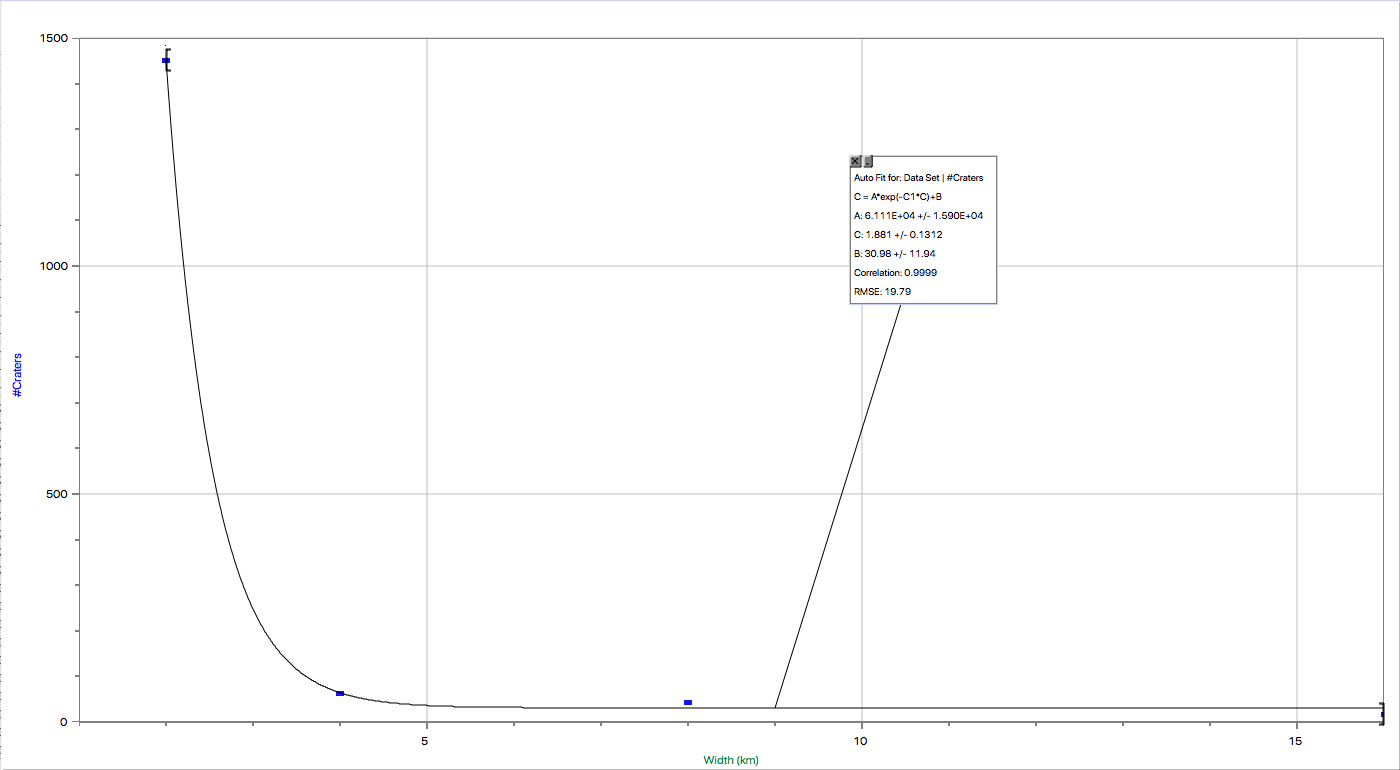
\includegraphics[width=0.85\textwidth]{4.png}
    \caption{Frequency of craters for various widths}
    \label{fig:3}
\end{figure}

\begin{figure}[H]
    \centering
    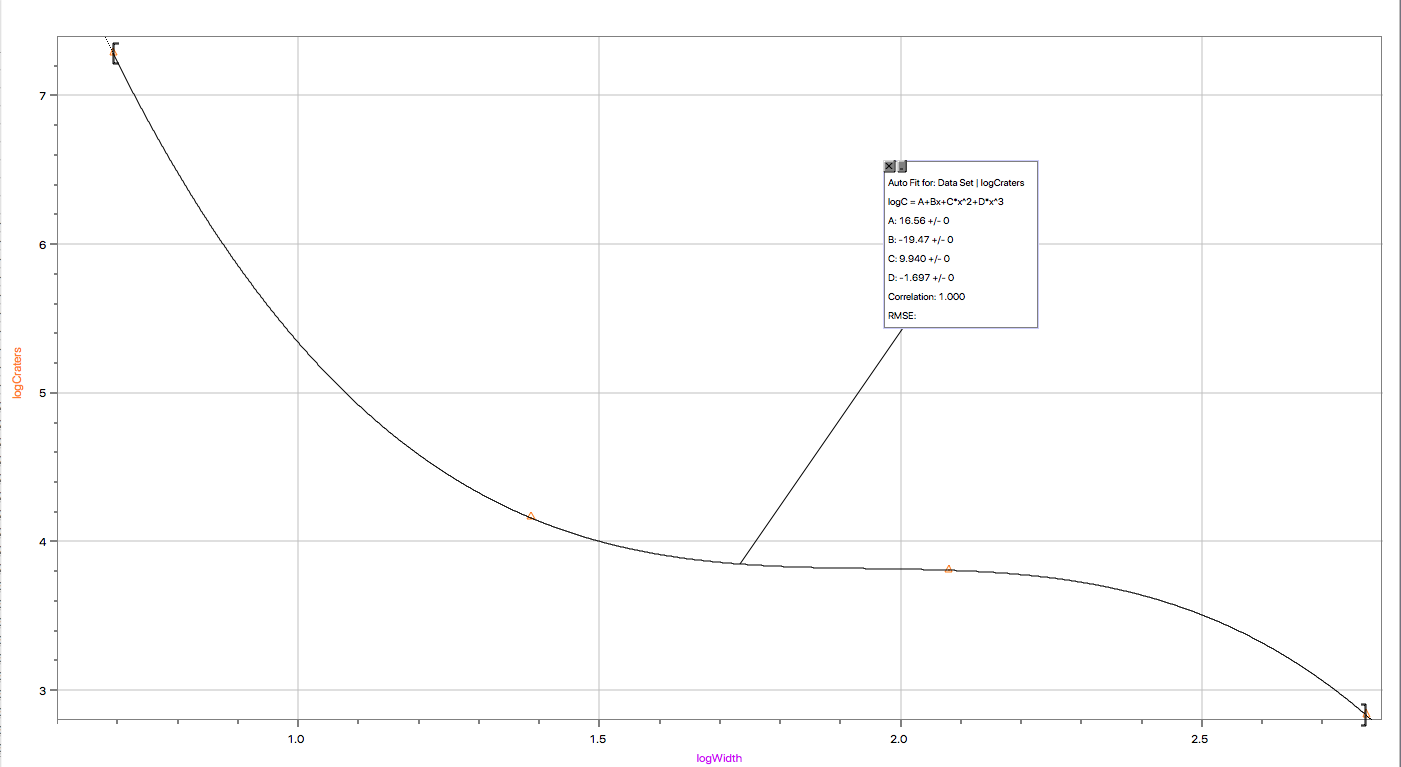
\includegraphics[width=0.85\textwidth]{3.png}
    \caption{log-log plot of crater Width vs frequenct}
    \label{fig:4}
\end{figure}


\section*{Conclusions and discussion}
It is apparent from Fig. 2 that there is a linear relationship between crater width and crater height. Craters with greater diameters have proportionally greater depths. The range of masses for the impacting asteroids was found to be between $~10^6$kg and $~10^{13}$ kg. From Fig. 4 and Fig. 5 it can clearly be seen that there is a far greater number of small craters on the moon than large. We estimate over 3000 craters of $D>16$km. This is an interesting image of what the Earth might look like were it not for seismic and volcanic activity. There is enormous room for error in this experiment, which is to be expected when the apparatus is photographs of a body $3.84 \times 10^5$m away. For greater precision we could have used photos with better resolution and smaller length conversion factors.



\end{document}
